% Homework template for Algorithm Analysis and Design
% UPDATE: September 20, 2019 by Xu Rongchen
\documentclass[a4paper]{article}
\usepackage{ctex}
\ctexset{
proofname = \heiti{证明} %% set proof name
}
\usepackage{amsmath, amssymb, amsthm}
% amsmath: equation*, amssymb: mathbb, amsthm: proof
\usepackage{moreenum}
\usepackage{mathtools}
\usepackage{url}
\usepackage{bm}
\usepackage{enumitem}
\usepackage{graphicx}
\usepackage{subcaption}
\usepackage{booktabs} % toprule
\usepackage[mathcal]{eucal}

\usepackage[thehwcnt = 2]{iidef} % set homework count
\usepackage{longtable}


\thecoursename{高等计算机网路}
\theterm{2020年秋季学期}
\hwname{论文阅读}
\slname{\heiti{解}}
\begin{document}
\courseheader
\theusername{徐荣琛}
\thestuno{2019214518}
\theinstitute{软件学院}

\info


  
  % \setlength{\itemsep}{3\parskip}
  %% Homework Start here:
  %% \item to enumerate the problem ID: Format as 'HomeworkID.ProblemID'
  %% \begin{solution} XXXX \end{solution} is to make a solution
  %% \begin{proof} XXXX \end{proof} is to make a proof
  %% Suggest to use \input{path} command
\vspace{-15pt}
\begin{center}
  \begin{tabular}{c|c} \toprule
    \textbf{专题} &TCP安全 \\\midrule
    \textbf{题目} &Off-Path TCP Exploits of the Mixed IPID Assignment\\
    \textbf{作者} &Feng X, Fu C, Li Q, Sun K, Xu K\\
    \textbf{会议} &ACM CCS 2020\\\bottomrule
  \end{tabular}
\end{center}
  
\vspace{20pt}
\setlength{\parindent}{2em}
本篇论文主要工作是研究了利用Linux下IPID分配规则漏洞进行TCP侧信道攻击。
本文提出的利用IPID规则漏洞进行TCP侧信道攻击主要包含有3个主要的步骤:
\begin{itemize}
  \item 伪装路由器向服务器发送虚假的ICMP分片要求(Fragmentation Needed)消息,使得
    服务器将IPID分配从基于每个套接字规则降低安全度到基于哈希计数器的规则;
  \item 利用哈希碰撞,使得攻击者能够和客户端之间共享同一个哈希计数器(通过观察攻击者与服务器
  间IPID计数器的变化发现);
  \item 通过观察攻击者与服务器间IPID计数器的变化发现,进一步推断连接的Sequence和
  ACK的窗口和编号等信息并进而进行侧信道攻击。
\end{itemize}

文章较为细致地介绍了攻击的具体流程并进行了一系列攻击的模拟实验,实验结果表明,基于Linux下
IPID分配规则漏洞进行TCP侧信道攻击具备了较为广泛的适用性和较高的成功率。

文章主要提出了两类的解决措施,一是改变通过DF字段识别TCP的方式避免被虚假的ICMP分片要求欺骗;
二是修改RST数据包的IPID分配方式,避免RST数据包的差异导致的信息侦测。
\begin{figure}[!htb]\centering
  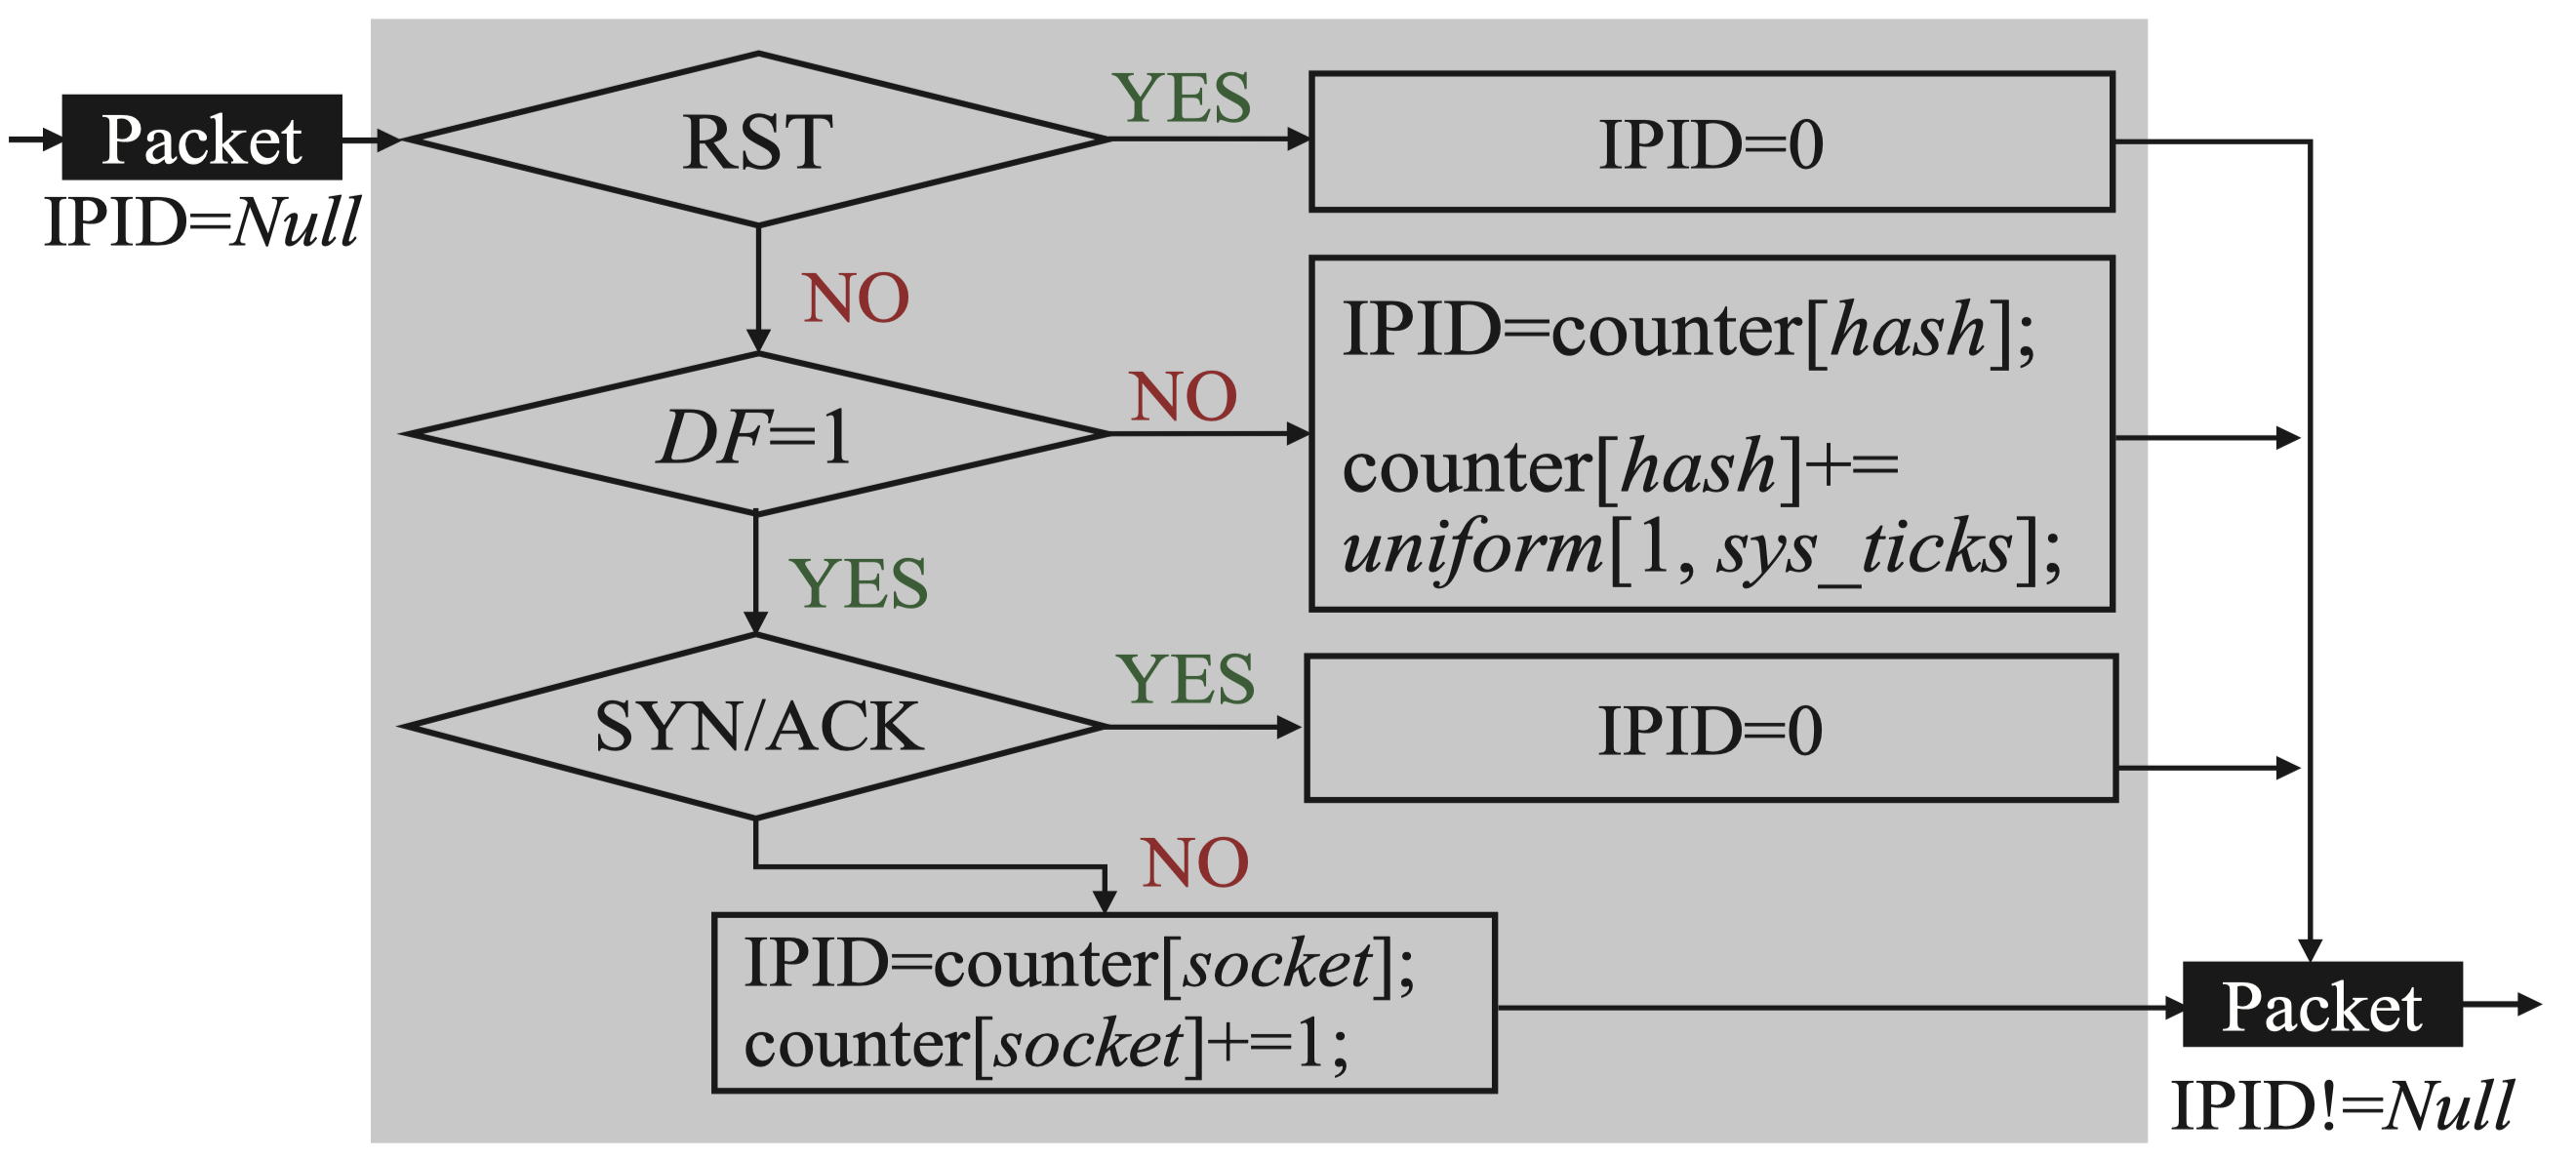
\includegraphics[scale=0.2]{figures/original.png}
  \caption{IPID分配规则示意图}
  \label{fig:ipid}
\end{figure}

在阅读论文的过程之中,
个人还想到了从掩饰IPID变化特征的角度上进行改良防范来自攻击者的观察。如图\ref{fig:ipid}所示,现有的
情况下,对应DF标识为0的情况下IPID的分配值直接来自于哈希计数器,而哈希计数器的变化是一个
1到$sys\_ticks$的均匀分布,这就导致了高频请求下$sys\_ticks$为1,计数器增加量固定是1,
而固定1的增量是整个漏洞的一个最关键的因素点所在,攻击者非常容易据此观察到IPID字段的变化规律。个人想到的改进方法是IPID的值并不直接等于
哈希计数器的计数值,而是外面再套一层随机排列,即:
$$\text{IPID} = \textsc{RandPerm}(counter[hash])$$
其中,$\textsc{RandPerm}$是预先生成的一个随机排列。在此方案下,由于IPID可观察到的变化是攻击者未知的一个
序列,则可以有效解决通过IPID值变化导致的潜在信息泄漏。如果要进一步避免潜在的观察风险,可以定期
(如IPID的空间用完时)变更随机排列的种子,同时需要一定程度上改动随机排列的规则,避免相邻的两个随机排列间存在过于接近
的相同IPID(例如对IPID的空间进行分组随机排列)。

\vspace{200pt}

\end{document}